\documentclass[11pt, twoside, listof=totocnumbered, bibliography=totocnumbered]{scrartcl}

%math
\usepackage{amsmath,amssymb,amstext}

%url
\usepackage{url}

%language
\usepackage{ucs}
\usepackage[utf8x]{inputenc}
\usepackage[T1]{fontenc}
\usepackage[ngerman, main=english]{babel}
\usepackage{blindtext}

%images
\usepackage{graphicx}

%header/footer
\usepackage[
bmargin=25mm, 
tmargin=20mm,
inner=50pt,
outer=80pt
]{geometry}
\usepackage{scrlayer-scrpage}
\usepackage{lastpage}

%arrows
\usepackage{textcomp}

\usepackage{multicol}

\usepackage{hyperref}

%code listings
\usepackage{caption}
\DeclareCaptionType{code}[Codebeispiel][Codebeispielverzeichnis] 

%code (C#)
\usepackage{listings}
\usepackage{xcolor}
\definecolor{bluekeywords}{rgb}{0,0,1}
\definecolor{greencomments}{rgb}{0,0.5,0}
\definecolor{redstrings}{rgb}{0.64,0.08,0.08}
\definecolor{grey}{rgb}{0.5,0.5,0.5}
\definecolor{types}{rgb}{0.17,0.57,0.68}
\usepackage{listings}
\lstset{language=[Sharp]C,
	captionpos=b,
	numbers=left, %Nummerierung
	numberstyle=\color{grey}\scriptsize,
	frame=lines, % Oberhalb und unterhalb des Listings ist eine Linie
	showspaces=false,
	showtabs=false,
	breaklines=true,
	showstringspaces=false,
	breakatwhitespace=true,
	escapeinside={(*@}{@*)},
	commentstyle=\color{greencomments},
	morekeywords={partial, var, value, get, set},
	keywordstyle=\color{bluekeywords},
	stringstyle=\color{redstrings},
	basicstyle=\ttfamily\small,
}
%\begin{lstlisting}[caption=a test for a C$^\sharp$ code, label=lst:test]
%code
%\end{lstlisting}

%bibliography
\bibliographystyle{alpha}

%Description environment
\usepackage[strict]{changepage}
\usepackage{framed}
\definecolor{formalshade}{rgb}{0.95,0.95,1}
\definecolor{darkblue}{rgb}{0,0,0.3}
\newenvironment{desc}{%
	\def\FrameCommand{%
		\hspace{1pt}%
		{\color{darkblue}\vrule width 2pt}%
		{\color{formalshade}\vrule width 4pt}%
		\colorbox{formalshade}%
	}%
	\MakeFramed {\advance\hsize-\width \FrameRestore}}%
{\endMakeFramed}

%bsubsection
\setcounter{secnumdepth}{4}
\setcounter{tocdepth}{4}

%custom commands
\newcommand{\br}{\hfill\\}
\newcommand{\phantomtitle}[1]{\noindent\textbf{\LARGE #1 }\\\br}
\newcommand{\bt}{{\color{grey}\blindtext}}
\newcommand{\cfct}[1]{\cite{#1}}
\newcommand{\imgct}[1]{(source: \cite{#1})}
\newcommand{\bld}[1]{\textbf{#1}}

%paragraph style
\setlength{\parindent}{0pt}
\setlength{\parskip}{1em}
\title{Device for digitizing materials}
\author{Niklas Hauber}
\date{\today{}, Linz} 
\begin{document}
\maketitle
Creation date of initial version: January 2, 2023\\
Publication date of initial version: January 2, 2023\\
Modification date of current version: \today{}\\

\section{Abstract}
Photometric stereo is a technique used to extract three-dimensional (3D) shape information of various materials and examine how these materials interact with light. This document serves as a defensive publication for a product designed to scan materials, analyzing their 3D shape, and their reflection, transmission, or emission of light. A key function of the product is to determine the parameters of a "Spatially Varying Bidirectional Reflectance Distribution Function" (SVBRDF).

The materials for scanning can be anything that manipulates light in some way, including but not limited to hot steel slabs, liquids, fabrics, leather, plants, rocks, skin, hair, and photoluminescent materials. The scanner deploys diverse light forms, each varying in form and/or spectral distribution, to illuminate the material. Utilizing a range of light sources mitigates any limitations that would be present if relying solely on a single light type. \cite{SURVEY}

More information on the current prototype can be found here: \\
\href{https://www.photometric.io/blog/material-scanner/}{https://www.photometric.io/blog/material-scanner/}

A solid introduction to photometric stereo can be found in this reference: \cite{SURVEY}

\section{Description}
The scanner comprises several optional components, including:
\begin{enumerate}
	\item One or more cameras that capture the light's interaction with the material. The use of multiple cameras enhances data availability and allows for a more accurate 3D model of the object through stereophotogrammetry. By integrating high frequency detail provided by the normal map derived from photometric stereo, an enhanced 3D representation of the object can be achieved. The cameras can either be fitted with a color filter array (CFA) or be monochrome, potentially with a filter wheel for superior quality images.
	
	\item Broadband point light sources, such as white LEDs, are typically used due to their affordability and ease of mathematical modeling. Despite these benefits, they may not perform well with glossy materials with low roughness, and hard shadows can cause artifacts unless properly managed. This can be mitigated by using them in greater number.
	
	\item Colored or spectrally variable point light sources, such as colored LEDs, lasers, or broadband light sources with filters, can provide useful information about the photoluminescence of the material. An inexpensive yet effective method to produce colored light involves collimating broadband light and diffract it using a diffraction grating causing different wavelengths to be at different angles from each other. This light can be focused onto a controllable optical slit. By varying the position and opening size of the slit, one can select a specific wavelength band. Ideally this light is then diffused via a normal diffuser or integrating sphere. See figure \ref{variable_light_source} for a drawing.

	\item Linear light sources, either broadband/white or colored/spectrally variable, can significantly improve the quality of scans for highly glossy materials. \cite{LINEAR_LIGHT}
	
	\item Area light sources can replace point light sources to aid with materials exhibiting low roughness. \cite{PS_AreaLights} A potentially more effective, albeit challenging, alternative could be to use point light sources behind a medium that scatters their light. This would result in lights having a falloff and could overlap each other. This means that any point on the hemisphere is covered by at least one light by some degree. If a glossy surface is illuminated by three lights with the same amount then the normal lies between those. This would allow scanning highly specular objects. See figure \ref{blurred_area_lights} for a drawing.
	 
	
	\item An area light source can be placed behind the material to measure translucency or transparency.
	
	\item All light sources can be paired with (linear/circular) polarizers to discern the specular and diffuse reflection of a material. Additionally, translucency and transparency can be separated using polarizers, as light waves directly passing through the material maintain polarization while scattered waves alter their polarization.
	
	\item Other 3D scanning technologies, such as structured light scanners or stereophotogrammetry (when using multiple cameras), can be used to capture a 3D representation of the material.
	
	\item An optical rangefinder can help adjust the focus of the camera lenses electronically or manually.
	
	\item Special lenses, like a tilt-shift lens, can be employed for scanning flat materials, allowing the image plane of a camera sensor to be parallel to the material, even if they are not physically aligned.
	
	\item To minimize stray light, the device's interior can be coated with a material that absorbs light well, such as black velvet. The scanner can be shielded by a cover or an enclosure to prevent the influence of ambient light. Alternatively, the scanning process can be performed in a dark environment.
	
	\item The light sources and cameras can be moved around the material, either physically or by using mirrors or other optical elements. Alternatively, the material itself can be moved while the light sources and cameras stay stationary. For instance, the material can be placed on a rotating platform or conveyor belt.
	
	\item A mobile device may be constructed by attaching the light sources to the multiple legs of the device, akin to a multi-legged tripod. A camera would be centrally mounted, facing downwards, and additional side-mounted cameras can be added to provide multiple viewing angles. This design would be both flexible and portable, with collapsible legs for ease of storage and transport.
	
	\item An alternative approach would involve attaching the scanner to a gantry. This could provide one to three-dimensional movement and more degrees of freedom for rotation. This capability would be especially useful for scanning larger materials or objects, where multiple scans across different areas are required. These scans can be subsequently merged to generate a comprehensive scan of the entire object. The same could be achieved by mounting the object to be scanned on a device with similar functionality, such as a gantry for adjusting the position or a tiltable rotary table for rotation, which is similar to devices used in 5-axis CNC mills.
	
	\item To mitigate the effects of any luminance instability from the light sources, a device can be directly illuminated to measure the intensity of the light. This data can then be used to adjust for any light source variations during the scanning process. The exposure of the device needs to be synchronized with the camera exposure. Alternatively, a spectrometer can be used to classify the spectral distribution of the light sources, which can further help to compensate for any instability in this distribution. This can also be used to monitor the long term instability of all light sources to find out when any lights should be replaced by new ones.
	
	\item Depending on the usage scenario and the available infrastructure, the scanner can be powered either by batteries or directly from an outlet. This flexibility allows the scanner to be used in a variety of settings and reduces the dependency on a constant power source.
\end{enumerate}
	
\section{Methodology}
The proposed scanning process involves several steps:

\begin{enumerate}
	\item Calibration: Calibration is performed to ascertain the camera's intrinsic properties (focal length, principal point, vignetting, lens distortion parameters, ...) and extrinsic properties (position and orientation in relation to the material). Furthermore, the position and brightness distribution of the light sources are also calibrated.
	\item Illumination and Capturing: The material is then illuminated by the light sources, and the cameras capture the resulting interaction between light and material. In a simple setup each image captures the object being illuminated by a single light. Optionally more images per light can be captured with varying cross or parallel polarization or different band pass filters in front of the camera and/or lights. Optionally this process can be repeated at different focus points to allow for focus stacking. All of this can then be repeated for different camera positions and rotations relative to the object to be scanned.
	\item Post-Processing: The captured images are processed to extract various material properties. The specific algorithms used will depend on the types of light sources and the properties of the material. The outcome of this step could include a normal map of the material's surface, its SVBRDF parameters, or a 3D model.
	\item Result Analysis: Finally, the processed data can be analysed or visualised, and used for various applications such as quality control, material design, or computer graphics rendering.
\end{enumerate}

\section{Capture and Processing Details}

\begin{enumerate}
	\item The scanning process involves capturing images of the reflection of light emitted by one or more light sources. A group of cameras simultaneously captures these reflections. The light sources can be modulated to produce a pattern or gradient in the reflected light. If there are multiple cameras and multiple light sources, the maximum total number of images taken for a single scan (assuming the material and camera remain stationary) equals the number of cameras times the number of light sources. This total is further multiplied by the number of filters if a filter wheel is employed.
	
	\item The images captured are processed by a computer, with the computations executed either on the CPU or GPU for efficient processing. The choice between the two will largely depend on the specific requirements of the computations and the capabilities of the hardware.
	
	\item The images may be transmitted to the computer directly from the cameras or, in the case of standalone cameras with onboard storage, the images can be first stored within the camera and then transferred to the computer for further processing.
	
	\item Light sources can be toggled on and off using a variety of methods. One such method employs MOSFETs paired with daisy-chained shift registers controlled by a microcontroller or computer. This system has the advantage of scalability. Other forms of communication, like I2C between the microcontroller and an LED controller, are also possible. Yet another alternative is to use one dimmable constant current controller for each LED. This allows for the implementation of multiple dimming methods such as analog, PWM, and shunt FET dimming. The specific dimming method can be dynamically chosen via software.
	
	\item Multispectral images can be acquired using multiple colored light sources or different filters. High color accuracy can be achieved by multiplying the acquired samples per pixel with a pre-calculated matrix. See figure \ref{multispectral_to_rgb}.
	
	\item Normals of the material can be calculated using the images of the specular reflection. By comparing these normals with those calculated from the diffuse reflection of the broadband or colored light sources, subsurface scattering parameters can be estimated. Once the normals from the specular reflections are obtained, solving for the subsurface scattering parameters directly (like via gradient descent) can be executed, but this may require more computational resources. \cite{SSS}
\end{enumerate}

The above details shed light on the in-depth process of capturing and processing images for material scanning. The scanner design, coupled with this comprehensive methodology, allows for accurate capture and analysis of a wide range of material properties.


\section{Future Scope and Potential Extensions}

While the current focus is on the primary objectives of the project, there are several potential enhancements and additional applications that could be explored in the future:

\begin{enumerate}
	\item \textbf{Portability:} Minimizing the weight of the scanner could transform it into a handheld device, offering enhanced convenience and portability. This could broaden its usage scenarios, such as field studies or on-site analysis.
	\item \textbf{Advanced Imaging:} The acquisition and separation of multiple reflections from various light sources in a single image could be achieved by using cameras fitted with polarization or color filters. This could involve employing a filter wheel or Color Filter Array (CFA). Having multiple polarized and/or colored light sources in different positions would enhance this setup. A beam splitter could be utilized for efficiency, allowing multiple cameras to capture images from the same perspective. The characteristics of the beam splitter could be adjusted based on the polarization or color of the light, possibly utilizing thin-film filters.
	\item \textbf{Digital Material Conversion:} The algorithm used for processing the acquired data could be adapted to convert existing digital materials into other formats. This could be achieved by rendering these materials in a virtualized version of the scanner setup. For instance, the properties of a Disney BRDF for a material could be calculated and converted even if the digital version is in another format.
	\item \textbf{GAN Network Enhancement:} A Generative Adversarial Network (GAN) could be trained on the resulting textures to improve perception. Ideally, the perceptual loss would be calculated on rendered images, which would require gradient backpropagation through the renderer. This could be achieved directly, through analytical approximations, or via trained neural networks to attain a good approximation.
	\item \textbf{Simplified Scanner:} A simpler scanner design with fewer light sources and potentially without polarization could be realized. To handle the reduced data, a neural network like a U-Net could be trained to predict the different textures. The network training could ideally be done using the results from a more complex scanner as ground truth. The input during training could be renders of the ground truth or a subset of images captured by the larger scanner.
	\item \textbf{Data Interpolation for Glossy Materials:} For highly glossy materials, normals and roughness values can be interpolated for pixels that did not contain enough reflected light to calculate the textures accurately. This can be done by setting a minimum specularity (F0) for the material and checking if the measured values align with a high enough roughness value that sufficiently illuminates the pixels. If a lower roughness value is necessary for the measured results, interpolation might be necessary. Once the areas for interpolation are identified, this can be done by examining the nearest patches of normals that did reflect enough light in any image for accurate calculation.
	\item \textbf{Augmented Reality Visualization:} Captured materials can be compared to the real samples using AR googles (like the Apple Vision Pro) to display a rendered version of the material next to the real one. For this an approximation of the environmental lighting is necessary, which can either be assumed fixed, estimated via machine learning solutions or measured using one or more cameras.
	\item \textbf{Joint Photogrammetry / Photometric Stereo Capture:} By photographing an object illuminated by multiple light sources from multiple directions, one has the data to do a photogrammetry workflow followed by calculating the material properties via photometric stereo for each camera angle and mapping those results onto the 3d object. Which is how existing approaches handle this. Another approach would be to have a software which first applies the photometric stereo step to get a set of material properties for each pixel and camera position. This would for example result in a normal map, albedo, roughness,... for each camera position. By aggregating all textures to a single multi-channel image, more robust features can be extracted to be used for a photogrammetry workflow. This photogrammetry workflow could be similar to the one used in Meshroom (\href{https://alicevision.org/\#photogrammetry}{https://alicevision.org/\#photogrammetry}) with the main difference that the input to the whole pipeline is a multi channel texture describing all material properties obtained by photometric stereo instead of normal photographs. An additional possible improvement could be to use the previously calculated normal maps (and/or calculated height maps by integrating the normal maps) to aid in the depth map estimation, which could potentially improve the quality of high frequency details in the 3d object. Optionally a post processing step could use all available view and light directions for each pixel to refine the material properties. Each step, namely the initial photometric stero solver, all steps of the photogrammetry pipeline (feature extraction, image matching, features matching, structure from motion, depth maps estimation, meshing and texturing) as well as the last postprocessing step can either be implemented by analytical/heuristical methods or by neural networks trained to fully or partly take care of this step.
\end{enumerate}

These potential extensions underline the versatility and scalability of the scanner system, paving the way for future advancements and wider applications in material scanning and imaging.

\section{Applications and Impact}
The proposed device offers broad applicability spanning across various domains. Its primary function lies in digitizing real-world materials and computing the parameters that describe these materials based on the Disney Bidirectional Reflectance Distribution Function (BRDF).\cite{DISNEY_BRDF} This ability to accurately capture and recreate the physical characteristics of a material digitally opens up new possibilities in fields such as computer graphics, virtual reality, and industrial design.

Moreover, the device's versatility extends beyond material digitization, making it an effective tool in various other fields. In the medical domain, it could potentially be used for skin scanning, providing crucial insights into skin health and abnormalities. For industrial applications, the device could serve as an optical inspection tool for surfaces such as steel slabs, aiding in quality control and defect detection.

\section{Acknowledgements and Legal Considerations}
The concepts and ideas presented here have been inspired by various research publications and other sources not all of which have been cited explicitly. This document serves as an informal exposition of a material scanner's concept rather than a formal scientific publication.

While the ideas listed here are open for anyone to utilize and adapt, it's crucial to be aware of existing patents that could potentially be infringed upon if all these ideas are implemented collectively. There is a plethora of patents related to the method of photometric stereo, some with very broad claims. Therefore, before implementing these ideas, thorough patent research and legal consultation should be undertaken to ensure compliance with all relevant intellectual property laws.

\newpage
\section{Tables \& Graphs}
\begin{figure}[h!]
	\begin{center} 
		\includegraphics[width=1\linewidth]{variable_light_source.png}
		\caption{Drawing of a variable wavelength light source} 
		\label{variable_light_source}
	\end{center} 
\end{figure} 
\begin{figure}[h!]
	\begin{center} 
		\includegraphics[width=1\linewidth]{blurred_area_lights.jpg}
		\caption{Visualization of overlapping blurred area lights. Each light is represented by a colored blurry point in the drawing to make it easier to understand, but should all be considered white lights.} 
		\label{blurred_area_lights}
	\end{center} 
\end{figure} 
\begin{figure}[h!]
	\begin{center} 
		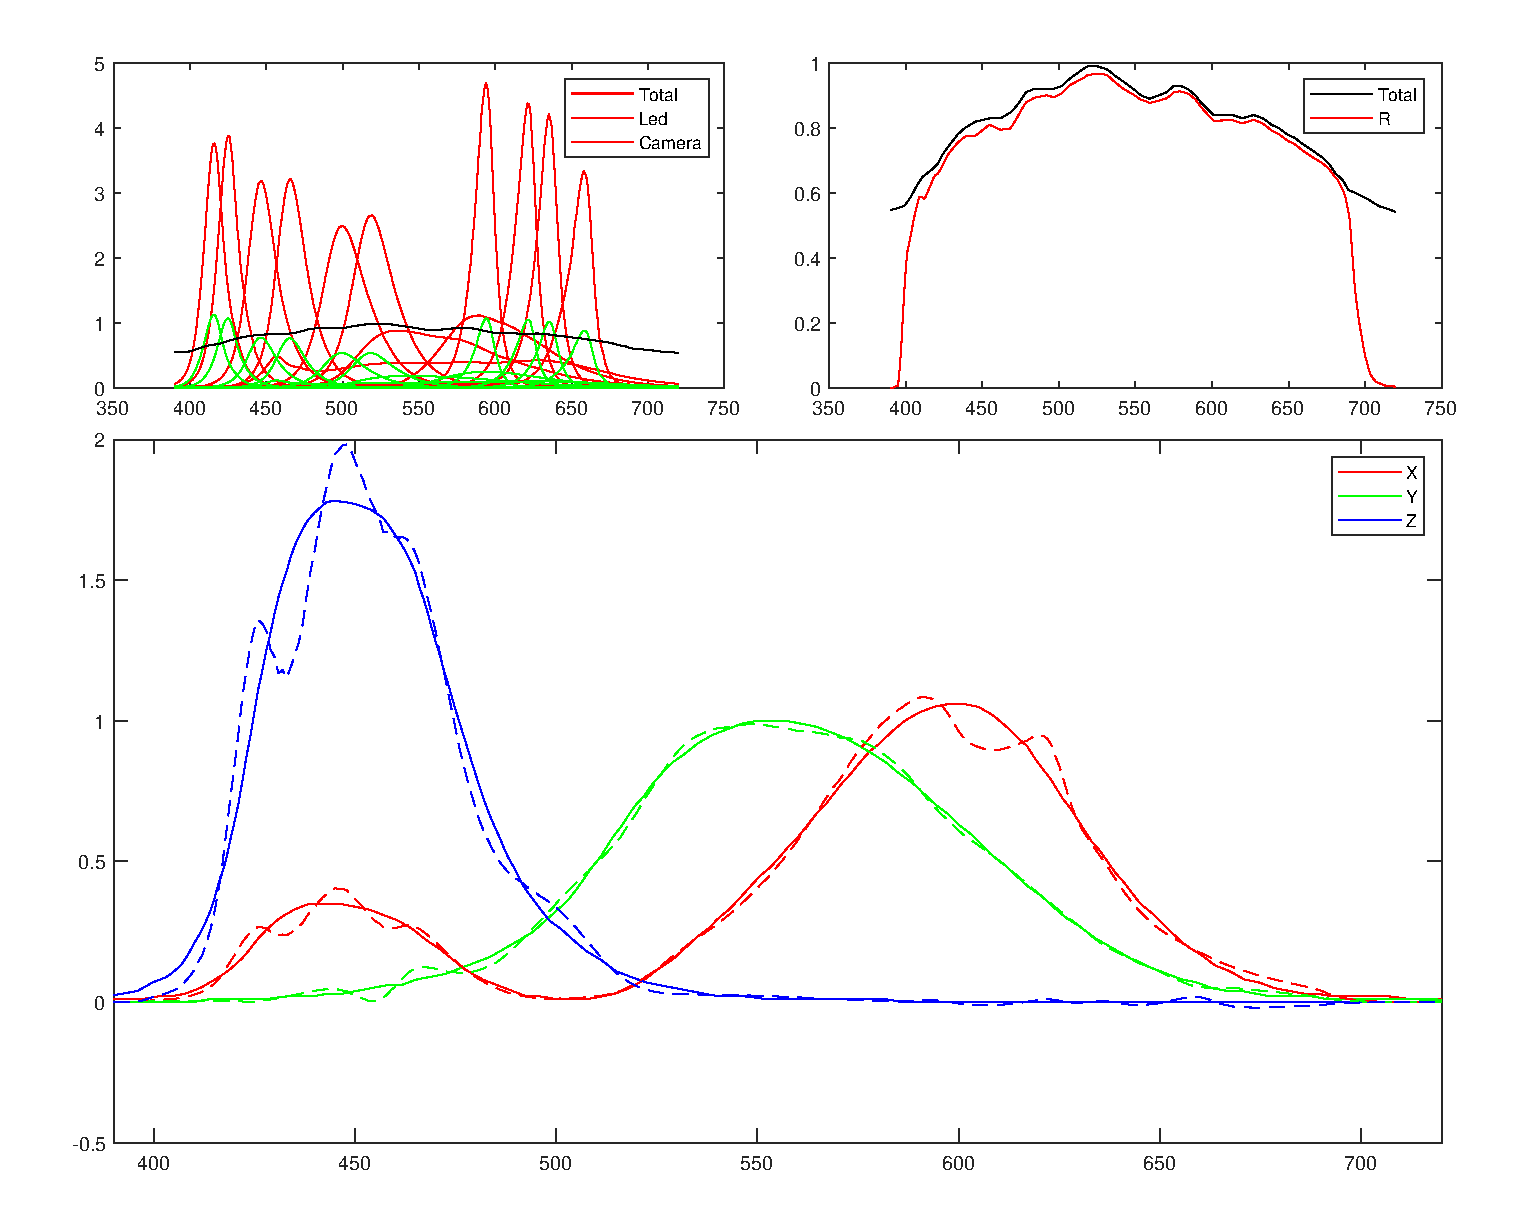
\includegraphics[width=1\linewidth]{chart.eps}
		\caption{Multispectral to RGB charts (top left: specular distribution of light sources, top right: specular response of camera, bottom: reference XYZ response combined with theoretical spectral response of merged images taken in combination with each led)} 
		\label{multispectral_to_rgb}
	\end{center} 
\end{figure} 
\newpage
\bibliography{TextureScanner.bib}
\vspace*{\fill}
\textsuperscript{\textcopyright} 2023 Niklas Hauber, All rights reserved.
\end{document}